\documentclass[a4paper,12pt]{article}
\usepackage[latin1]{inputenc}
\usepackage[spanish]{babel}
\usepackage{bm}
\usepackage{graphicx}
\usepackage{amsmath}
\setlength{\textheight}{235mm}
\setlength{\textwidth}{168mm}
\setlength{\oddsidemargin}{0pt}
\pagestyle{empty}
\begin{document}
\mbox{}\vspace*{-45mm}

{\centering
{\small\sc Escuela Técnica Superior de Ingenieros de Caminos, Canales y
Puertos (Madrid)}\\*[4mm]
{\Large\bf Método de los Elementos Finitos (Curso 22-23)}\\*[4mm]
Ejercicio 3: Elasticidad lineal \\*[4mm]

}

\vspace{3mm}

%%%%%
Una placa de aluminio, con módulo de elasticidad $E=70$ GPa y coeficiente de Poisson $\nu=0.33$, está sometida a una presión uniforme de $50$ MPa en los lados verticales. La placa tiene un espesor de $5$ mm. Dada la simetría existente, se recomienda analizar una cuarta parte del modelo. Se considerará la hipótesis de tensión plana. Para el mallado, considerar los siguiente:
\\

{\bf NOTAS:}
\begin{enumerate}
\item Para el cuarto de círculo, usar un mallado {\em Seed Edges, Method/By number, Bias/none, Sizing Controls/Number of elements: 15}
\item Para los bordes izquierdo, superior e inferior usar un mallado {\em Seed Edges, Method/By number, Bias/single, Sizing Controls/Number of elements: 20,  Sizing Controls/Bias ratio: 5}
\item Para el borde derecho, usar un mallado {\em Seed Edges, Method/By number, Bias/none,$ $Sizing Controls/Number of elements: 20}
\item En {\em Mesh Controls}, usar una forma de elemento triangular y malla estructurada.
\item El tipo de elemento a utilizar será {\em CPS3}.
\end{enumerate}
\begin{center}
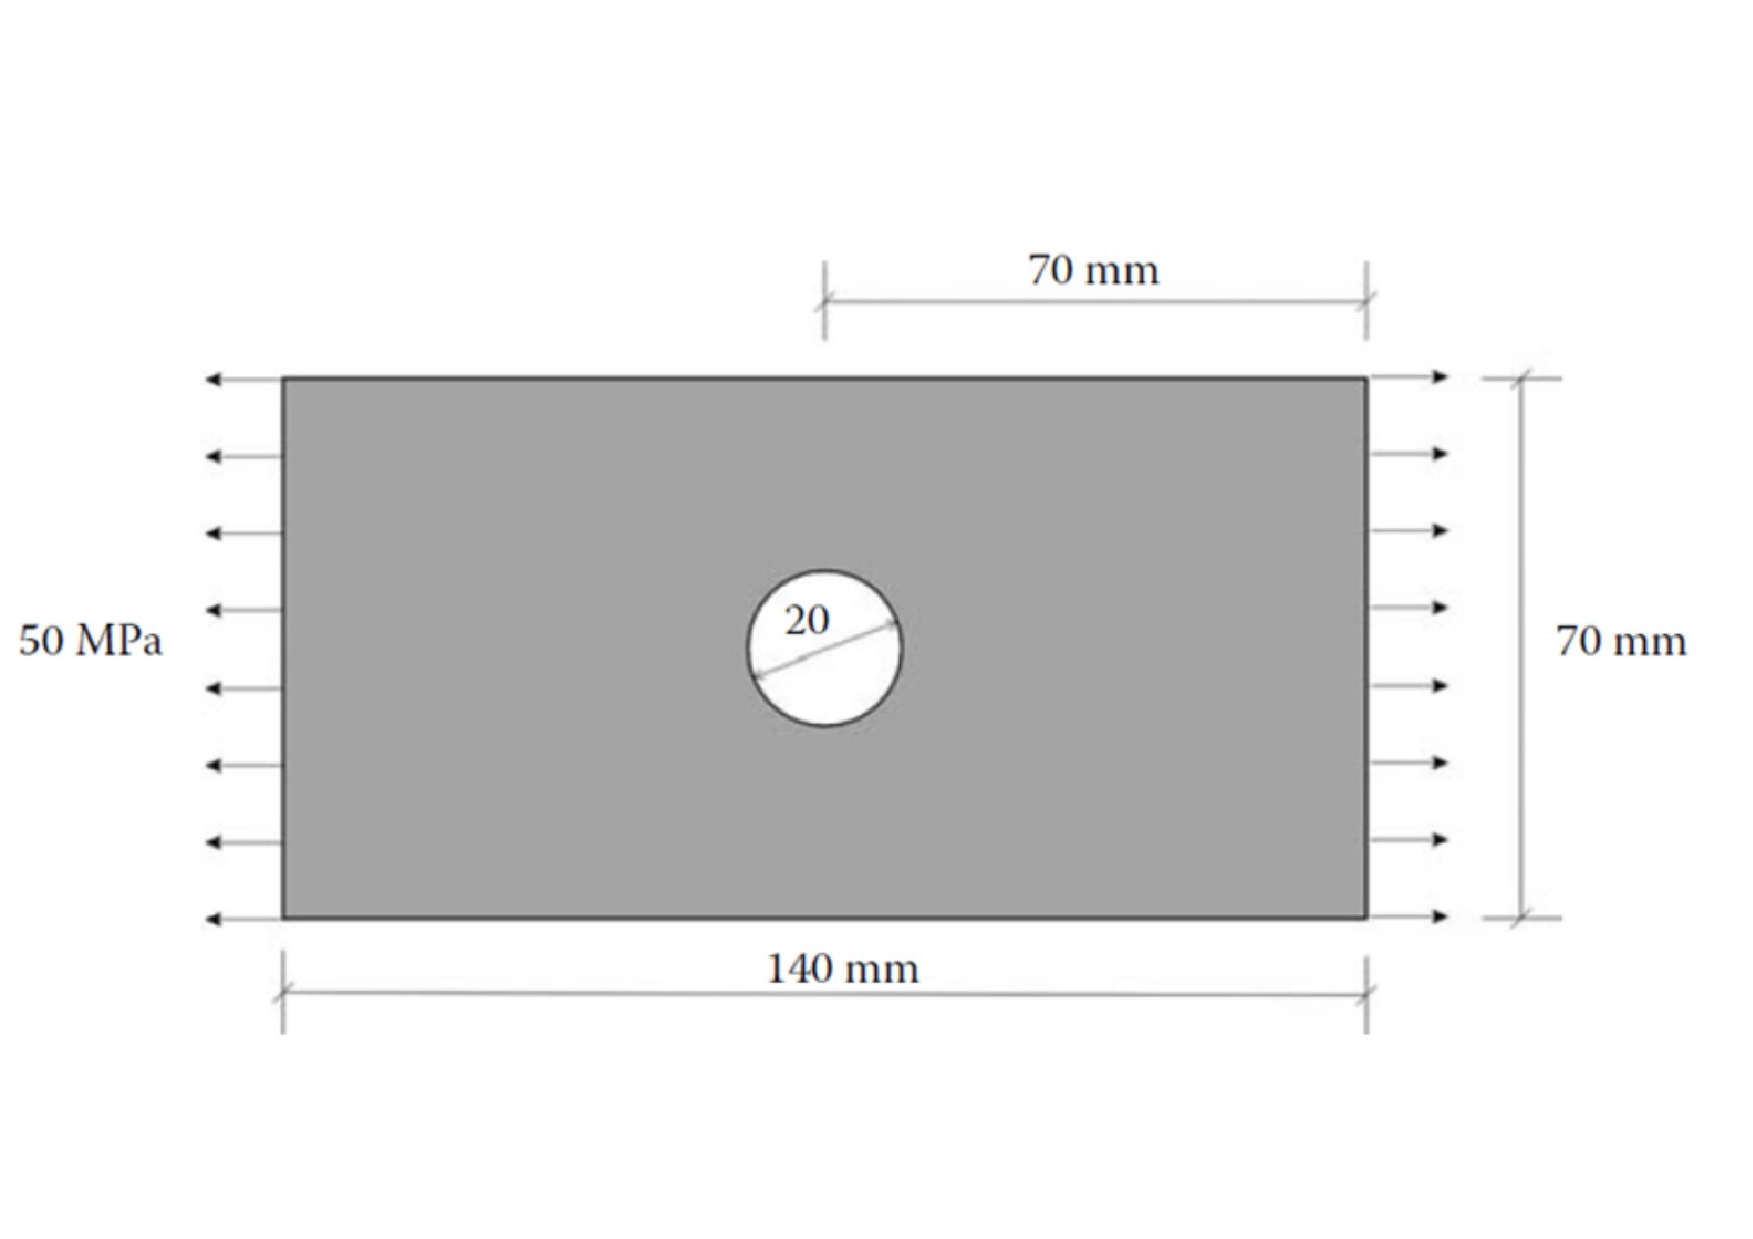
\includegraphics[width=0.70\textwidth]{figura}
\end{center}

\end{document}
